%% LaTeX-Beamer template for KIT design
%% by Erik Burger, Christian Hammer
%% title picture by Klaus Krogmann
%%
%% version 2.1
%%
%% mostly compatible to KIT corporate design v2.0
%% http://intranet.kit.edu/gestaltungsrichtlinien.php
%%
%% Problems, bugs and comments to
%% burger@kit.edu
\pdfminorversion=4

\documentclass[18pt]{beamer}

\usepackage[utf8]{inputenc}
\usepackage{listings}
%% SLIDE FORMAT

% use 'beamerthemekit' for standard 4:3 ratio
% for widescreen slides (16:9), use 'beamerthemekitwide'

\usepackage{templates/beamerthemekit}
% \usepackage{templates/beamerthemekitwide}

%% TITLE PICTURE

% if a custom picture is to be used on the title page, copy it into the 'logos'
% directory, in the line below, replace 'mypicture' with the 
% filename (without extension) and uncomment the following line
% (picture proportions: 63 : 20 for standard, 169 : 40 for wide
% *.eps format if you use latex+dvips+ps2pdf, 
% *.jpg/*.png/*.pdf if you use pdflatex)

\titleimage{../media/background}

%% TITLE LOGO

% for a custom logo on the front page, copy your file into the 'logos'
% directory, insert the filename in the line below and uncomment it

\titlelogo{logo}

% (*.eps format if you use latex+dvips+ps2pdf,
% *.jpg/*.png/*.pdf if you use pdflatex)

%% TikZ INTEGRATION

% use these packages for PCM symbols and UML classes
% \usepackage{templates/tikzkit}
% \usepackage{templates/tikzuml}

\usepackage{hyperref}
\usepackage{color}

% speech bubbles
\usepackage{tikz}
\usetikzlibrary{shapes.callouts}
\usetikzlibrary{arrows,positioning}
\usetikzlibrary{calc}

% rotations
\usepackage{rotating}

% strike through in math mode
\usepackage{cancel}

% for embedded video
\usepackage{multimedia}

% for multiline comments
\usepackage{verbatim} 

\usepackage{color}

% the presentation starts here

\title[Lambda Spiel]{Spass beim Lernen der Lambdakalkülprinzipien}
%\subtitle{Spielend die Denkweise des Programmierens lernen}
\author{PSE 2014/2015}

\institute{Farid Elhaddad | Florian Fervers | Kai Fieger | Robert Hochweiss | Kay Schmitteckert}
\date{\today}

\beamertemplatenavigationsymbolsempty

\begin{document}

% change the following line to "ngerman" for German style date and logos
\selectlanguage{ngerman}

\begin{frame}
	\titlepage
\end{frame}

\begin{frame}{Ziel}
	\begin{itemize}[<+->]
	\item Kindern im Grundschulalter das Konzept des $\lambda$-Kalküls nahebringen
	\item Lernfortschritt erreichen durch Spielfreude und "`Gamification"'
	\item Kindgerechte Bedienung
	\item Funktionen für begleitende Lehrpersonen
	\end{itemize}
\end{frame}

\begin{frame}{Spielelemente}
	\centering
	\begin{tabular}[h]{l | l}
	Lambda-Kalkül & Lamb.da Analogie \\
	\hline
	Variable & 
\includegraphics[height=1.cm]{pictures/gem_blue} \\
	Abstraktion & 
\includegraphics[height=1.cm]{pictures/lamb_blue} \\
	Klammerung & 
\includegraphics[height=1.cm]{pictures/lamb_white}
	\end{tabular}
\end{frame}

\begin{frame}{Beispielterm}
	$(\textcolor{blue}{\lambda x. } \textcolor{red}{\lambda y. y} \ (\textcolor{blue}{x \ x})) \ \textcolor{green}{z}$ \\
	\vspace{0.3cm}
	
\includegraphics[scale=1.8]{pictures/lamb_long_blue} \hspace{0.8cm}  
\includegraphics[scale=0.5]{pictures/gem_green} \\
	\vspace{0.3cm}
	
\includegraphics[scale=1.7]{pictures/lamb_red} \hspace{0.1cm} 
\includegraphics[scale=1.7]{pictures/lamb_white}\\
	\vspace{0.3cm}
	\hspace{0.5cm} 
\includegraphics[scale=0.5]{pictures/gem_red} \hspace{0.05cm} \hspace{1.7cm} 
\includegraphics[scale=0.5]{pictures/gem_blue} \hspace{0.05cm} 
\includegraphics[scale=0.5]{pictures/gem_blue} \\
\end{frame}

\begin{frame}{Spielregeln}
	\centering
	\begin{tabular}[h]{l | l}
	Lambda-Kalkül & Lamb.da Analogie \\
	\hline
	$\beta$-Reduktion & Verzauberungsregel \\
	$\alpha$-Konversion & Umfärbungsregel \\
	Einfache Klammerung & 1. Regel für Lämmer ohne Zauberstab \\
	Linksassoziativität & 2. Regel für Lämmer ohne Zauberstab
	\end{tabular}
\end{frame}

\begin{frame}{Editormodus}
	Zum Erstellen eines Terms durch den Spieler
	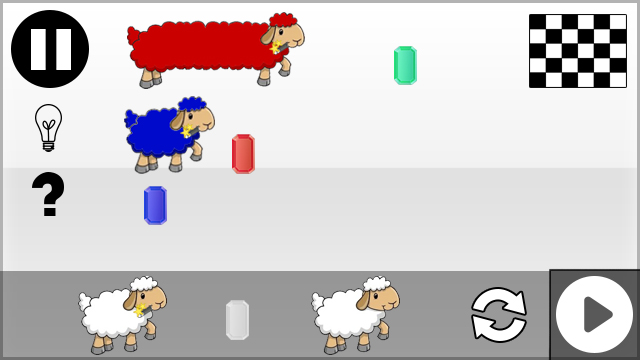
\includegraphics[scale=0.5]{../gui/_jpeg/game}
\end{frame}

\begin{frame}{Reduktionsmodus}
	Zum automatischen Ausführen der Spielregeln
	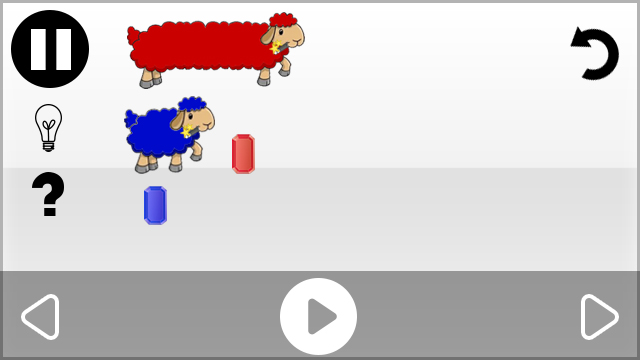
\includegraphics[scale=0.5]{../gui/_jpeg/game_play_started}
\end{frame}

\begin{frame}{Leveltypen}
	\begin{itemize}
	\item Eingabe-Bestimmung: Erstellen eines $\lambda$-Terms, der nach Anwenden der Spielregeln zu einem gegebenen Term wird
	\item Ausgabe-Bestimmung: Erstellen eines $\lambda$-Terms, der aus einem gegebenen Term durch Anwenden der Spielregeln hervorgeht
	\end{itemize}
\end{frame}

\begin{frame}{Motivation}
	Elemente zur Verbesserung der Spielfreude und des Lernfortschritts:
	\begin{itemize}[<+->]
	\item Münzen: Erhalten nach erfolgreichem Levelabschluss, eintauschen im Shop gegen Belohnungen
	\item Erfolge: Angezeigt nach bestimmten Leistungen des Spielers
	\item Sandbox: Ermöglicht das freie Austoben im Lambda-Kalkül
	\end{itemize}
\end{frame}

\begin{frame}{Shop}
	Zum Eintauschen von Münzen gegen Belohnungen
	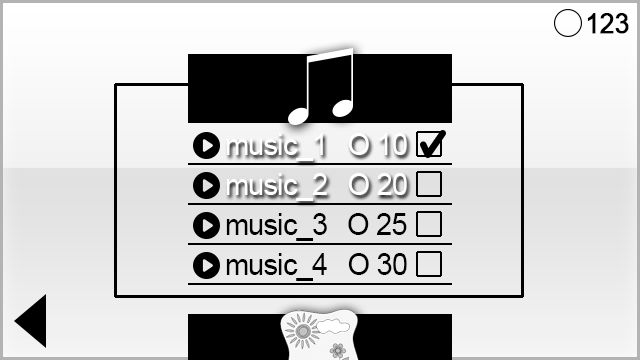
\includegraphics[scale=0.5]{../gui/_jpeg/shop_popup}
\end{frame}

\begin{frame}{Betreuer}
	Elemente für Eltern und Lehrer:
	\begin{itemize}[<+->]
	\item Lehrermodus: Zeigt im Editor-/Reduktionsmodus den aktuellen Term in Lambda-Kalkül Schreibweise an
	\item Statistik: Gibt Einsicht in das Spielverhalten der Kinder
	\end{itemize}
\end{frame}

\begin{frame}
	\centering
	\huge Vielen Dank für Ihre Aufmerksamkeit!
\end{frame}

\end{document}
